\section{Separated index windows}\label{sec:windows}

We first assign a finite block of dyadic indices to every edge of an
ordered tree.  Gaps between the blocks will let small translations
preserve earlier grid cells.  Each block will also be long enough to
control all resolutions needed below its child.  These two properties
will serve different purposes in the random construction.

\subsection{The tree and the window lengths}

Fix $p\in(0,1)$.  Choose integers $M\ge2$ and $d\ge1$ such that
\begin{equation}
 \frac{p(M-1)}2\ge10,
 \qquad
 (1-2^{1-M})^d<p.
 \label{eq:tree-parameters}
\end{equation}
Such choices can be made in this order: the first inequality holds for
large enough $M$, after which $0<1-2^{1-M}<1$ permits the second choice.
Let $\mathcal T$ be the complete ordered tree of height $d$ in which each
internal vertex has $M$ children.  Its root has height $d$, its leaves
have height $0$, and the children of an internal vertex $P$ are
$P_1,\ldots,P_M$.  Write $e=(P,i)$ for the edge from $P$ to $P_i$.
The finite total number of edges is
\[
 K=\sum_{\ell=1}^d M^\ell.
\]
List the edges in the following preorder: for each vertex $P$, list
$(P,1)$ and all edges below $P_1$, then $(P,2)$ and all edges below
$P_2$, and so on.  Thus an edge together with all edges below its child
forms one consecutive block in the list.

Choose an integer $g\ge1$ such that
\begin{equation}
 K2^{2-g}<p.
 \label{eq:gap-budget}
\end{equation}
This choice depends only on the already fixed tree.  We will leave $g$
unused indices between consecutive windows.

The $M-1$ nondefault child windows of a node, each of length $r$, will
together supply $(M-1)r$ random tests at a fixed scale $t\in[1,2]$.
The exponential factor in the next inequality will bound
the probability that all these tests fail. The preceding factor will
bound the size of a finite list of scale values that represents every
possible collection of local grid keys as $t$ varies. Making their
product small will control all normalized scales by a finite union
bound; Sections~\ref{sec:routing} and~\ref{sec:scales} prove these two
bounds.

Choose an integer $r_*\ge1$ such that, for every integer
$r\ge r_*$,
\begin{equation}
 20Mr(1+2^{2r+2})
       \exp\!\left(-\frac{p(M-1)}2r\right)<p.
 \label{eq:entropy-budget}
\end{equation}
For completeness, the left side is at most $100M e^{-7r}$ when $r\ge1$:
use \eqref{eq:tree-parameters},
$1+2^{2r+2}\le5e^{2r}$, and $r\le e^r$.
Hence any integer $r_*>\log(100M/p)/7$ works simultaneously for all
larger $r$.  The uniformity will allow us to enlarge windows as needed.

We assign a window length $r_h$ to edges whose parent has height $h$.
At the same time we compute the span $\sigma_h$ of all windows in a
subtree of height $h$, including the gaps between them.  Starting with
$\sigma_0=0$, define successively for $h=1,\ldots,d$
\begin{equation}
 \begin{split}
 r_h&=\max\{r_*,g+\sigma_{h-1}\},\\
 \sigma_h&=
 \begin{cases}
 Mr_1+(M-1)g,&h=1,\\
 M(r_h+g+\sigma_{h-1})+(M-1)g,&h\ge2.
 \end{cases}
 \end{split}
 \label{eq:window-recursion}
\end{equation}
This is a finite bottom-up recursion: $r_h$ depends only on lengths
already chosen below height $h$.  In particular, the choice of $g$ did
not depend on the sizes of these lengths.

Now place the actual integer windows in the edge preorder, starting at
$3$.  An edge $e$ from height $h$ receives
$W_e=\{a_e,\ldots,b_e\}$ with $b_e=a_e+r_h-1$; if $f$ immediately
precedes $e$, set $a_e=b_f+g+1$.  Put
\[
 \mathcal N=\bigcup_{e\in\mathcal T}W_e,
\]
where the union is over the edges of the tree.  The span interpretation
of \eqref{eq:window-recursion} follows by induction.  At height $1$
there are $M$ windows and $M-1$ gaps.  At height $h\ge2$, each child
block consists of an incoming window of length $r_h$, one gap, and a
subtree block of span $\sigma_{h-1}$; there are another $M-1$ gaps
between these child blocks.

For an edge $e=(P,i)$, let $b_e^*$ be the largest window endpoint among
$e$ and all edges below $P_i$.  If $P$ has height $h=1$, this block
consists only of $e$, and its span is $r_1$.  If $h\ge2$, its span is
$r_h+g+\sigma_{h-1}$.  Therefore in both cases
\begin{equation}
 b_e^*-a_e+1\le r_h+g+\sigma_{h-1}\le2r_h.
 \label{eq:padding}
\end{equation}
In particular, \eqref{eq:entropy-budget} applies to every length $r_h$,
while \eqref{eq:padding} bounds a whole child block in terms of its
incoming window.  All edges, including those with child index $M$,
receive windows under this construction.

The padding bound has a specific purpose: the range of window indices
from $a_e$ through $b_e^*$ in a child block is controlled by the length
of its incoming window. The gaps have a different role, established
next: for most centers, translations indexed by a later window preserve
the earlier cells used in the routing decisions. These
are the two deterministic inputs to the routing and scale-counting
arguments.

\begin{figure}[htbp]
\centering
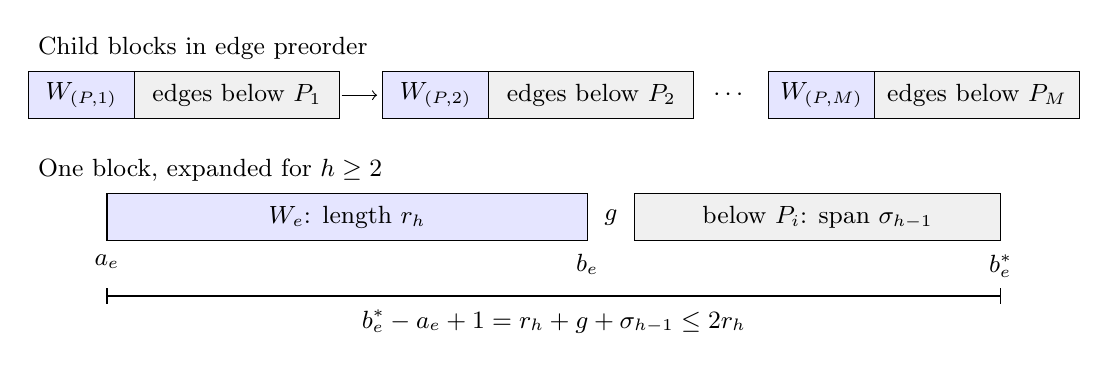
\begin{tikzpicture}[x=1cm,y=1cm,font=\small]
  \node[anchor=west] at (0,2.5) {Child blocks in edge preorder};
  \foreach \start/\index in {0/1,4.5/2,9.4/M}{
    \fill[blue!10] (\start,1.6) rectangle (\start+1.35,2.2);
    \fill[gray!12] (\start+1.35,1.6) rectangle (\start+3.95,2.2);
    \draw (\start,1.6) rectangle (\start+3.95,2.2);
    \draw (\start+1.35,1.6)--(\start+1.35,2.2);
    \node at (\start+.675,1.9) {$W_{(P,\index)}$};
    \node at (\start+2.65,1.9) {edges below $P_{\index}$};
  }
  \draw[->] (3.98,1.9)--(4.43,1.9);
  \node at (8.89,1.9) {$\cdots$};
  \node[anchor=west] at (0,.95) {One block, expanded for $h\ge2$};
  \fill[blue!10] (1,.05) rectangle (7.1,.65);
  \fill[gray!12] (7.7,.05) rectangle (12.35,.65);
  \draw (1,.05) rectangle (7.1,.65);
  \draw (7.7,.05) rectangle (12.35,.65);
  \node at (4.05,.35) {$W_e$: length $r_h$};
  \node at (7.4,.35) {$g$};
  \node at (10.025,.35) {below $P_i$: span $\sigma_{h-1}$};
  \node[anchor=north] at (1,0) {$a_e$};
  \node[anchor=north] at (7.1,0) {$b_e$};
  \node[anchor=north] at (12.35,0) {$b_e^*$};
  \draw (1,-.65)--(12.35,-.65);
  \draw (1,-.55)--(1,-.75);
  \draw (12.35,-.55)--(12.35,-.75);
  \node[anchor=north] at (6.675,-.7)
    {$b_e^*-a_e+1=r_h+g+\sigma_{h-1}\le2r_h$};
\end{tikzpicture}
\caption{Each edge window precedes the windows below its child, and
the child blocks are listed in order.  The lower diagram includes the
gap before a nonempty child subtree.  An edge into a leaf has no
following subtree or internal gap.  Lengths are schematic.}
\label{fig:windows}
\end{figure}


\subsection{Earlier grid cells remain unchanged}

For every nonnegative integer $b$, define the periodic cell key
\begin{equation}
 J_b(z)=\left\lfloor2^{b+2}\{z\}\right\rfloor,
 \qquad \{z\}=z-\lfloor z\rfloor.
 \label{eq:grid-key}
\end{equation}
Its boundaries on the real line form the lattice
$\Gamma_b=2^{-(b+2)}\mathbb Z$.  In particular, every integer is a
boundary.  Cells are half-open on the right, so a boundary belongs to
the cell starting there.  The grids are nested: for $B\ge b$,
\begin{equation}
 J_b(z)=\left\lfloor\frac{J_B(z)}{2^{B-b}}\right\rfloor.
 \label{eq:grid-nesting}
\end{equation}
This follows by writing $2^{B+2}\{z\}=J_B(z)+\varepsilon$ with
$0\le\varepsilon<1$ and dividing by the integer $2^{B-b}$.

We seek centers for which translations indexed by one window preserve
every earlier grid key.  For a noninitial window $W_e$, let $b'$ be the
endpoint of the immediately preceding window, and put
$\delta_e=2^{1-a_e}$.  Call $x$ \emph{stable} if, for every such window,
\begin{equation}
 (x,x+\delta_e]\cap\Gamma_{b'}=\varnothing.
 \label{eq:stable-definition}
\end{equation}
Let $G$ denote the set of stable centers.  The intervals in
\eqref{eq:stable-definition} are taken on the real line, so crossings
of an integer are included without a separate convention on the circle.

\begin{lemma}\label{lem:stable}
The set $G$ is measurable and $1$-periodic, and $\rho(G^c)<p$.
For every $x\in G$, every window $W_e$, every $n\in W_e$, every
$t\in[1,2]$, and every window $W_f$ earlier than $W_e$,
\begin{equation}
 J_{b_f}(x+t2^{-n})=J_{b_f}(x).
 \label{eq:stable-keys}
\end{equation}
These assertions include centers lying on grid boundaries.
\end{lemma}

\begin{proof}
For a fixed noninitial window, the centers violating
\eqref{eq:stable-definition} are exactly
\[
 E_e=\bigcup_{\beta\in\Gamma_{b'}}[\beta-\delta_e,\beta),
\]
because $\beta\in(x,x+\delta_e]$ if and only if
$\beta-\delta_e\le x<\beta$.  This is a measurable periodic set.
Since $a_e=b'+g+1$,
\[
 2^{b'+2}\delta_e=2^{2-g}<p/K<1.
\]
Thus these intervals have disjoint interiors modulo one.  There are
$2^{b'+2}$ of them per period, each of length $\delta_e$, and hence
$\rho(E_e)=2^{2-g}$.  The complement of $G$ is the union of these sets
over the $K-1$ noninitial windows.  Consequently
\[
 \rho(G^c)\le(K-1)2^{2-g}<p.
\]
This also proves measurability and periodicity of $G$.

Now fix the data in \eqref{eq:stable-keys}.  If $W_e$ is the first
window, there is no earlier $W_f$.  Otherwise
$0<t2^{-n}\le2^{1-a_e}=\delta_e$, so stability implies that the
interval $(x,x+t2^{-n}]$ contains no boundary of $\Gamma_{b'}$.
Both endpoints therefore have the same $J_{b'}$ key.  This remains true
when $x$ itself is a boundary, since it belongs to the cell on its
right; landing on a boundary at a positive displacement has been
excluded.  An integer cannot lie in this interval either, so passing
to periodic keys introduces no additional case.  Finally, every earlier
window satisfies $b_f\le b'$, and \eqref{eq:grid-nesting} gives
\eqref{eq:stable-keys}.
\end{proof}

The tree, all windows, and $G$ are now fixed before any random choices.
The key agreement concerns earlier windows only.  This is the property
that will preserve the required earlier decisions while allowing tests
at the current window's finer resolution.
